\begin{figure}[tp]
	\centering
	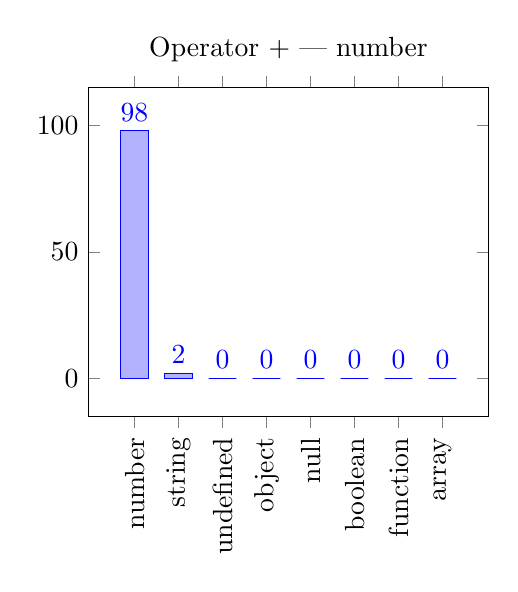
\begin{tikzpicture}
		\begin{axis}[
			ybar,
			title=Operator + | number,
			width=0.55\textwidth,
			ybar=0pt,
			ymax=100,
			enlargelimits=0.15,
			legend style={at={(0.5,-0.2)}, anchor=north,legend columns=-1},
			symbolic x coords={number,string,undefined,object,null,boolean,function,array},
			xtick=data,
			nodes near coords, 
			nodes near coords align={vertical},
			x tick label style={rotate=90,anchor=east},
		]
		\addplot coordinates {
			(number, 98)
			(string, 2)
			(undefined, 0)
			(object, 0)
			(null, 0)
			(boolean, 0)
			(function, 0)
			(array, 0)
		};
		\end{axis}
	\end{tikzpicture}
	%
	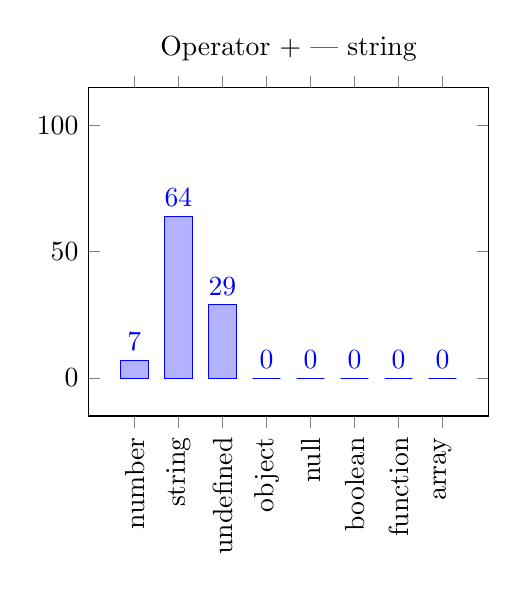
\begin{tikzpicture}
		\begin{axis}[
			ybar,
			title=Operator + | string,
			width=0.55\textwidth,
			ybar=0pt,
			ymax=100,
			enlargelimits=0.15,
			legend style={at={(0.5,-0.2)}, anchor=north,legend columns=-1},
			symbolic x coords={number,string,undefined,object,null,boolean,function,array},
			xtick=data,
			nodes near coords, 
			nodes near coords align={vertical},
			x tick label style={rotate=90,anchor=east},
		]
		\addplot coordinates {
			(number, 7)
			(string, 64)
			(undefined, 29)
			(object, 0)
			(null, 0)
			(boolean, 0)
			(function, 0)
			(array, 0)
		};
		\end{axis}
	\end{tikzpicture}

	\caption[Usage distribution for operator +]{\textbf{Usage distribution for operator \mintinline{text}{+}} - Both graphs were made by fixing the type of one of the operands. If a value is used with the operator \mintinline{text}{+} and the other operand is a \mintinline{text}{number}, the graph on the left should be used. If the second operand is a \mintinline{text}{string}, the graph on the right should be used.
	}

	\label{fig:type-inference-proposal-scoring-plus}
\end{figure}